\section{CUDA 工具包概述}

欢迎大家。今天我们将深入探讨 CUDA 工具包。CUDA 工具包是 GPU编程领域的基石，正在革命性地改变高性能计算和深
度学习应用。CUDA（Compute Unified Device Architecture，统一计算设备架构）是英伟达的
并行计算平台。这个工具包不仅仅是一套工具的集合，更是开启英伟达GPU 巨大潜力的大门。让我们探索其关键组件，并了解它们如
何使我们能够充分利用 GPU 计算的全部能力。

\begin{figure}
    \centering
    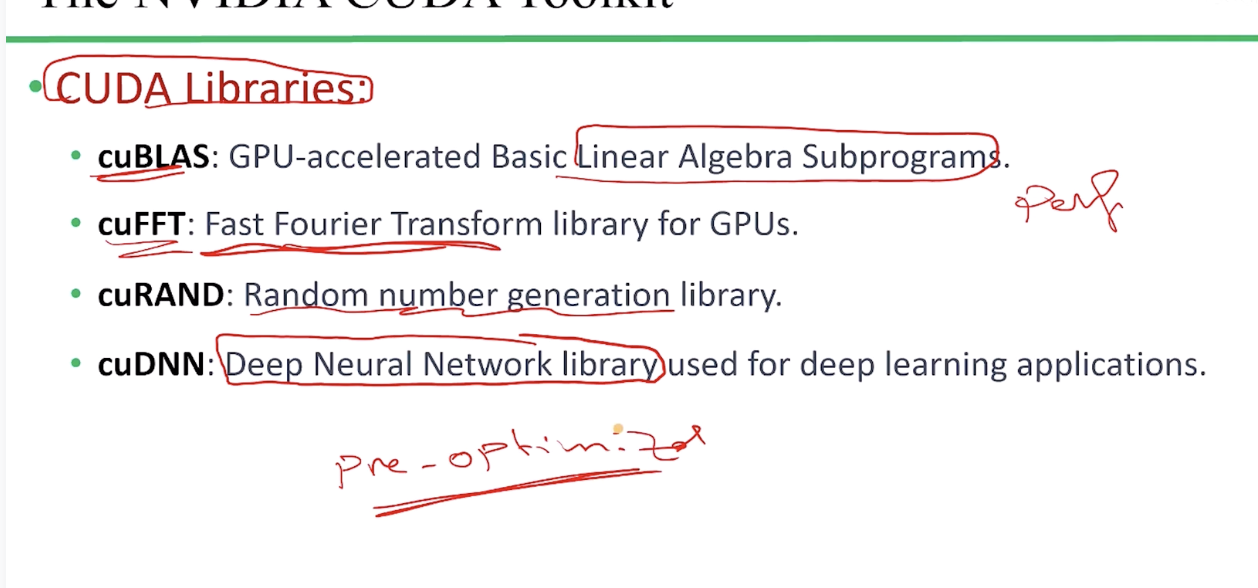
\includegraphics[width=0.75\linewidth]{resources/cuda-057.png}
    \caption{}
    \label{fig:placeholder}
\end{figure}

\subsection{nvcc编译器}

CUDA 开发的核心是 CUDA 编译器，即 \texttt{nvcc}编译器。它供开发人员、研究人员以及专业人士使用，
以简化从简单的 CUDA 编码到复杂 GPU应用程序的一切工作。该编译器是将高级 CUDA 代码转换为 GPU 可理解形
式的关键：它可以将 CUDA代码转换为与各种英伟达架构兼容的 PTX 代码。简而言之，\texttt{nvcc} 编译器
用于将 CUDA代码转换为可以在 GPU 上高效运行的可执行文件。

\subsection{优化库}

CUDA 拥有一套优化库的支持，每个库都有其专门用途。例如，\textbf{cuBLAS} 和\textbf{cuFFT}分别在线性代数
和快速傅里叶变换运算方面表现突出。这些库经过高度优化，能显著提升性能。此外还有\textbf{curand} 库，专门用于随机数生成；
以及 \textbf{cuDNN}库，这是一个为神经网络加速设计的深度学习库。这些库是高效 GPU编程的支柱，提供了预先优化的即用型函数，节省开发时间并增强性能。


\begin{figure}
    \centering
    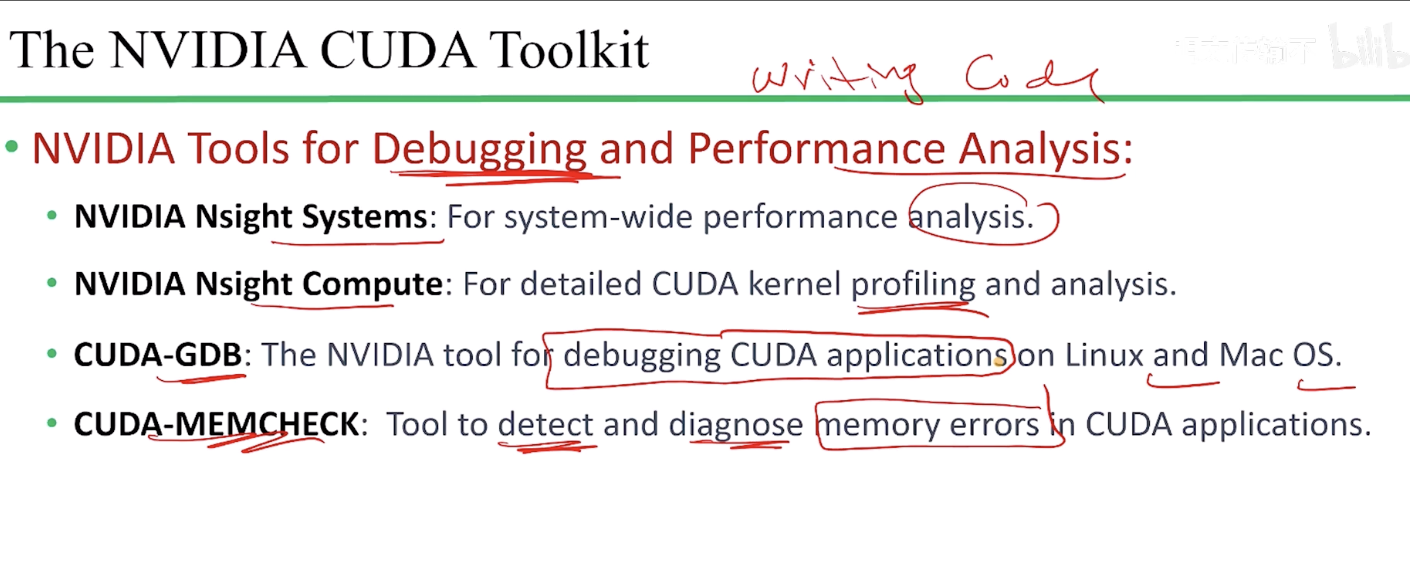
\includegraphics[width=0.75\linewidth]{resources/cuda-058.png}
    \caption{}
    \label{fig:placeholder}
\end{figure}

\subsection{运行时API}

CUDA 工具包还提供了运行时 API（RuntimeAPI），用于管理设备初始化、内存分配以及内核启动。它们对于管理应
用程序与 GPU 的交互至关重要。例如，对于 CPU和 GPU 之间的内存操作或数据传输，我们可以使用以下 API 函数：

\begin{itemize}
    \item \texttt{cudaMalloc}：在 GPU 设备上分配指定大小的内存。这类似于标准 C 语言中的 \texttt{malloc}，但专用于 GPU 而非 CPU 内存分配。
    \item \texttt{cudaMemcpy}：用于在主机（CPU）和设备（GPU）之间复制数据。
\end{itemize}

以上是运行时 API 函数的两个典型示例。
\subsection{调试与分析工具}

在这张幻灯片中我想强调，对于 GPU应用程序来说，工作不止于编写代码，还关乎确保效率和稳定性。这就是为什么英伟达工具包含了强大的工具：
\begin{itemize}
    \item \textbf{Nsight Systems} 和 \textbf{Nsight Compute}：用于分析和剖析应用程序的性能。
    \item \textbf{cuda-gdb}：提供在 Linux 和 macOS 操作系统上调试 CUDA 应用程序的强大环境。
    \item \textbf{cuda-memcheck}：专门用于检测和诊断内存问题的工具。
\end{itemize}
所有这些工具共同提供了一个全面的环境，不仅用于编写代码，还用于完善和优化 GPU 加速应用程序。

\begin{figure}
    \centering
    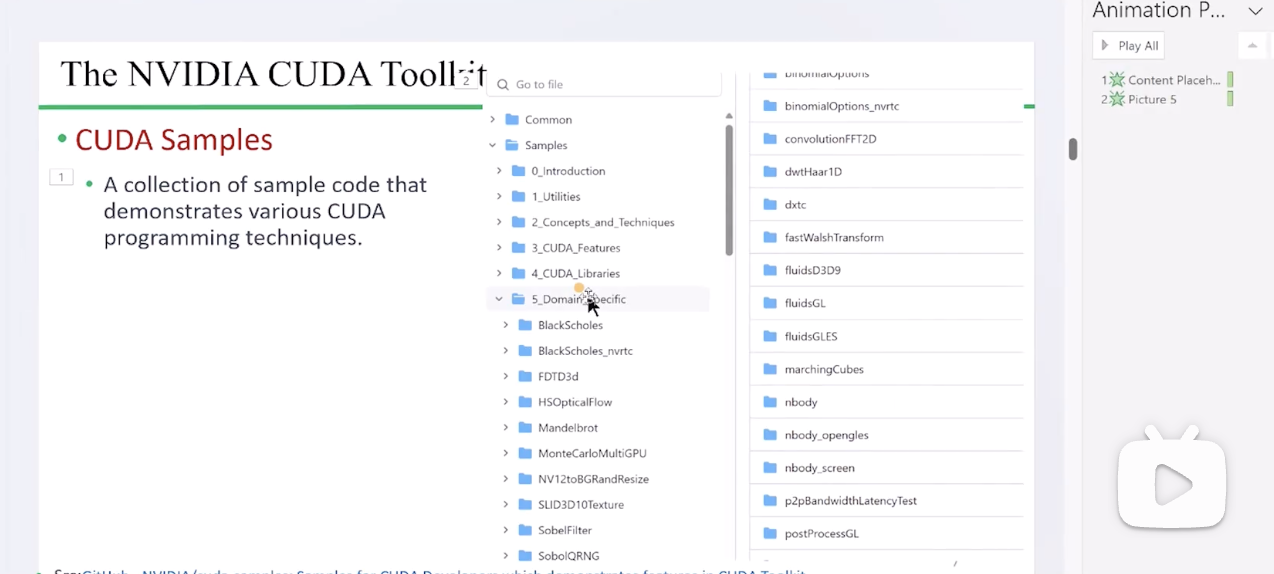
\includegraphics[width=0.75\linewidth]{resources/cuda-059.png}
    \caption{}
    \label{fig:placeholder}
\end{figure}


\subsection{示例代码}

CUDA 工具包附带了一套丰富的示例代码。这些示例不仅仅是代码，更是实用的指南，阐明了各种 CUDA编程技术，从基本概念
到高级操作，涵盖了广泛的场景和应用案例。这些示例可以提供对高效 CUDA编程的宝贵见解，提供一种实用的学习体验，补充理论
知识。

在本文章的最后，我想总结：CUDA 工具包不仅仅是编译 GPU 应用程序的编译器，或是编写 CUDA程序的编辑器。它是一
个综合平台，包含了编写、编辑、编译和剖析 GPU 应用程序所需的一切。
